\documentclass[handout]{beamer}
\usepackage{beamerthemesplit}
\usepackage{pgfpages}
\usetheme{Madrid}
\title[MANET Model and Simulation Design]{Dynamic MANET Model and Protocol \\ Simulation Design Plan}

\usepackage{mathptmx}
\usepackage[scaled=.90]{helvet}
\usepackage{courier}
\usepackage[T1]{fontenc}

%%\pgfpagesuselayout{4 on 1}[letterpaper,border shrink=5mm]

\institute[RIT]{}
\date{August 9, 2011}
%\subtitle{}
\author{Christopher A. Wood}
%\institute[]{}
%\date{}
\begin{document}

\begin{frame}
  \titlepage
  \begin{center}
	  %\textbf{caw4567@rit.edu}
	\end{center}
\end{frame}

%\begin{frame}
%  \frametitle{Outline}
%  \tableofcontents
%  % You might wish to add the option [pausesections]
%\end{frame}

%\section{Finite Field Basics}
\begin{frame}
 \frametitle{Simple MANET topology}
 \begin{center}
  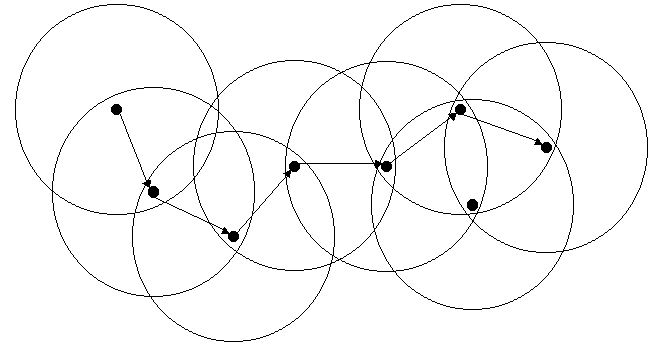
\includegraphics[width=75mm]{ad_hoc_net.jpg}
 \end{center}
\end{frame}

%\begin{frame}
% \frametitle{Complexity can increase...}
% \begin{center}
%  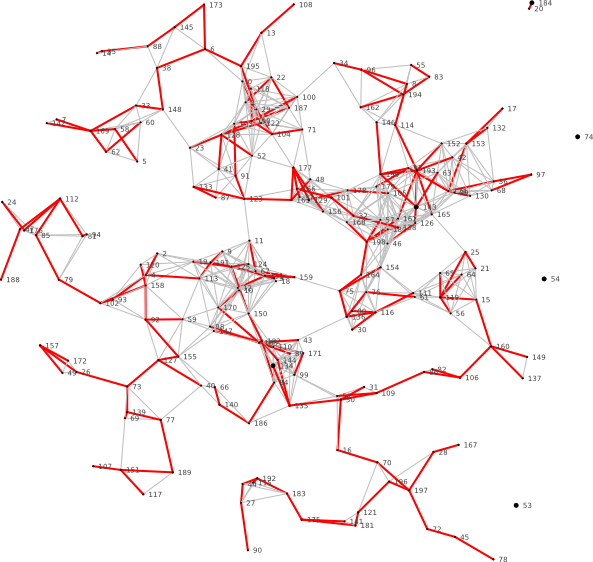
\includegraphics[width=75mm]{2Trees-1.png}
% \end{center}

%\end{frame}

\begin{frame}
 \frametitle{Node communication}
 \begin{center}
  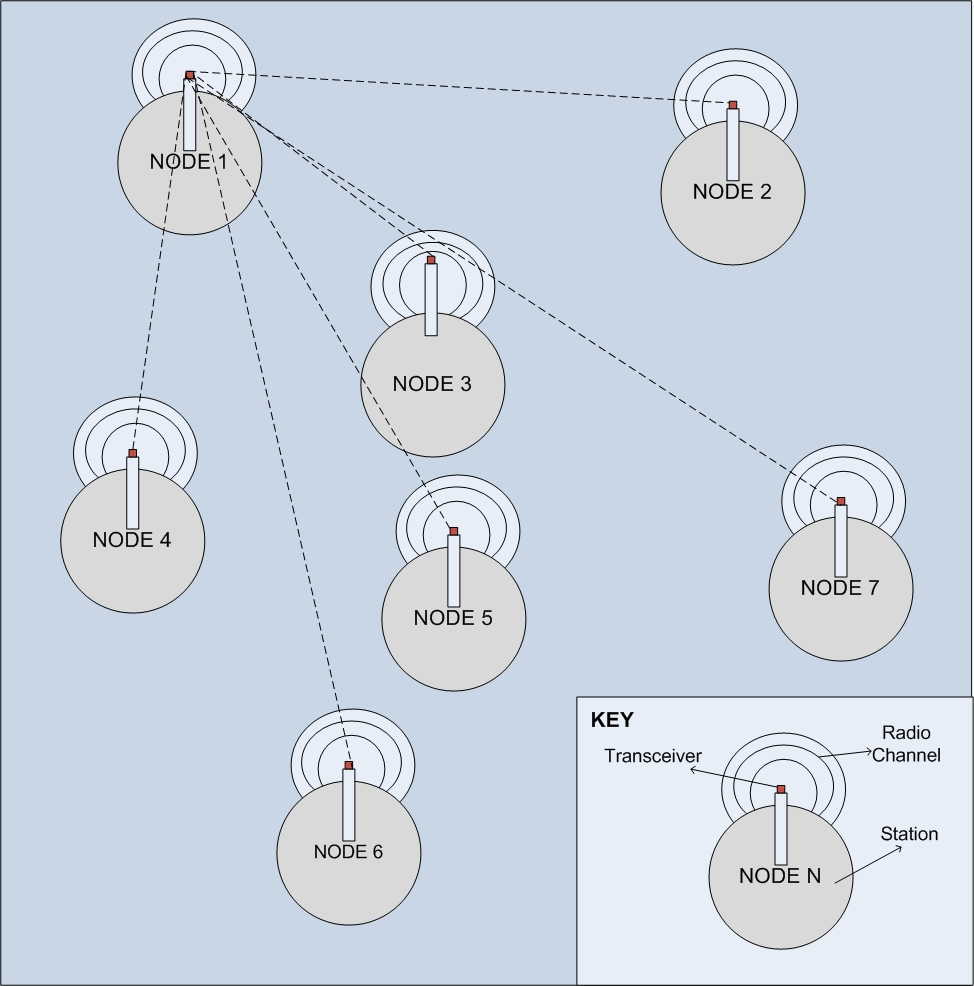
\includegraphics[width=75mm]{wireless_structure.jpg}
 \end{center}
\end{frame}

\begin{frame}
 \frametitle{Properties of dynamic MANETs}
 \begin{itemize}
  \item No pre-existing infrastructure in place for communication
  \item Nodes self-configure and arrange themselves in groups as they move around the grid
  \item Each node must be able to act as a router to forward data by other nodes
  \item Nodes are burdened with computational and power constraints
 \end{itemize}
 \begin{center}
  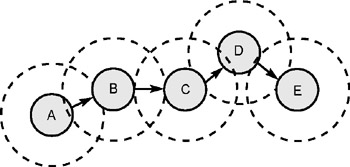
\includegraphics[width=70mm]{groups.jpg}
 \end{center}
\end{frame}

\begin{frame}
 \frametitle{Framework features}
 \begin{itemize}
  \item Support for configurable channels and environments for simulation
  \item Effective communication API to allow for emphasis on protocol algorithms and development
  \item Statistical data collection in both the physical communication and protocol layers of the model
 \end{itemize}
\end{frame}

\begin{frame}
 \frametitle{Framework features (continued)}
 \begin{itemize}
  \item Reusable cryptographic engine to provide standard primitives (hashing, encryption/decryption, etc)
  \item Abstract protocol classes to allow for specialized functionality for future protocols
  \item Script-driven configuration, execution, and analysis (preferably written in Python due to existing mathematical libraries and tools)
 \end{itemize}
\end{frame}

\begin{frame}
 \frametitle{Generic framework processes} 
 \begin{center}
  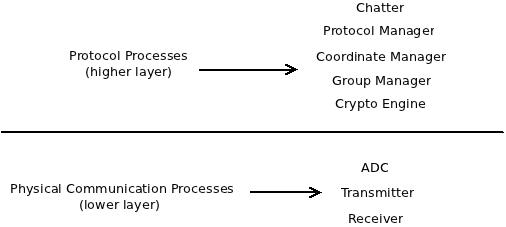
\includegraphics[width=100mm]{processes.jpeg}
 \end{center}

 All processes support \textbf{inheritance} for more specialized functionality, if needed

% \begin{columns}[c]
% 
%    \column{2.0in}
%    Communication-oriented (low layer)
%      \begin{itemize}
%        \item ADC
%        \item Transmitter
%        \item Receiver
%      \end{itemize}
%  
%    \column{2.0in}
%    Protocol-oriented (high layer)
%     \begin{itemize}
%      \item Chatter
%      \item CoordinateManager
%      \item GroupManager
%      \item ProtocolManager
%      \item CryptoEngine
%     \end{itemize}
% 
%  \end{columns}
\end{frame}

\begin{frame}
 \frametitle{Physical communication processes}
 \begin{itemize}
  \item \textbf{ADC} - Interprets incoming packets according to the physical 
properties of the channel (i.e. distinguishes legitimate signals from noise)
  \item \textbf{Transmitter} - Sends packets (retrieved from the internal packet 
queue) and messages to nearby nodes in the network
  \item \textbf{Receiver} - Forwards data retrieved from the network to the ADC
for verification and the protocol layer for processing
 \end{itemize}
\end{frame}

\begin{frame}
 \frametitle{Protocol processes}
 \begin{itemize}
  \item \textbf{Chatter} - Generates chatter data to be sent to processes (basically, the test driver)
  \item \textbf{Coordinate Manager} - Periodically generates coordinate messages to send to nearby nodes in the network and manages the neighbor table
  \item \textbf{Group Manager} - Manages the internal group table according to the proximity of nearby nodes
and members of the node group that are synchronized for communication
  \item \textbf{Protocol Manager} - Drives the main key management protocol
  \item \textbf{Crypto Engine} - Handles the primitive cryptographic operations (e.g. encryption/decryption, hashing, etc)
 \end{itemize}

Each process will manage the formation of its own packets (e.g. GKM messages are generated by the Protocol Manager)
\end{frame}

\begin{frame}
 \frametitle{Internal node structure}
 \begin{center}
  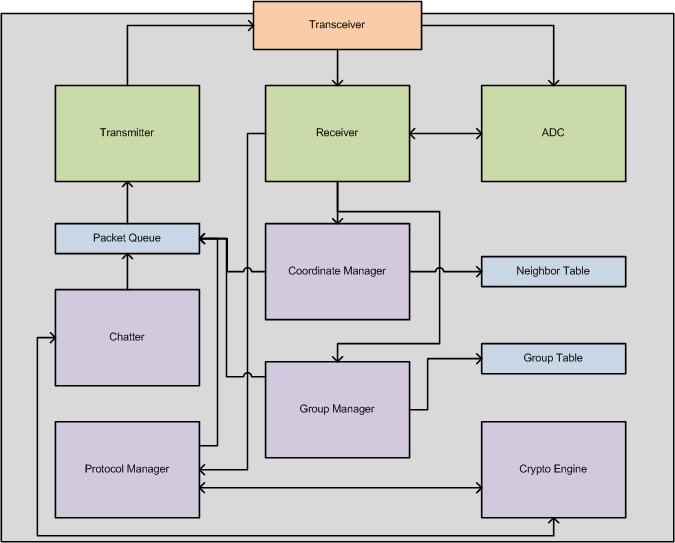
\includegraphics[width=85mm]{dynamic_node.jpg}
 \end{center}
\end{frame}

%%TODO: simulation parameters are going to be on separate document, printed out for adjustments/feedback from the group

\begin{frame}
 \frametitle{Expected output}

\begin{center}
The following statistical data will be collected from each simulation using SIDE random variables
\end{center}

 \begin{columns}[c]
 
    \column{2.0in}
    \textbf{Communication-oriented statistics:}
      \begin{itemize}
        \item Packet and message transmission time
        \item Overall and inter-node packet and message transmission delays
        \item History of SNR, BER, and other related signal data for each node due to environment and unrelated traffic
      \end{itemize}
  
    \column{2.0in}
    \textbf{Protocol-oriented statistics:}
     \begin{itemize}
      \item Frequency of group formations and modifications
      \item Computational overhead for protocol operations 
      \item Protocol message transmission time throughout groups
     \end{itemize}
  \end{columns}

\end{frame}

\begin{frame}
 \frametitle{Plugging in specific protocols}
 
Our first target is Professor Kaminsky's Automatic Group Key Management protocol, which requires the following additions to the model:

\begin{enumerate}
 \item Implement the AES, SHA-256, and RSA primitive operations inside the Crypto Engine process
 \item Add the radio unique IDs and GKM pairs for each node to the configuration file (this data is initialized at startup)
 \item Extend the Protocol Manager and Group Manager processes to support the new group formation/modification and key exchange operations
 \begin{itemize}
  \item This includes adding the functionality to build the packets correctly, as per the specficication of the protocol
 \end{itemize}
 \item Add the ability to support both static and dynamic groups
 \begin{itemize}
  \item Dynamic groups require the implementation of some spanning tree formation algorithm to aid the tree multicast transmission process
 \end{itemize}
\end{enumerate}
 
\end{frame}


\end{document}